%
% buchcover.tex -- Cover für das Buch Felder
%
% (c) 2018 Prof Dr Andreas Müller, Hochschule Rapperswil
%
\documentclass[11pt]{standalone}
\usepackage{tikz}
\usepackage{times}
\usepackage{geometry}
\usepackage[utf8]{inputenc}
\usepackage[T1]{fontenc}
\usepackage{times}
\usepackage{amsmath,amscd}
\usepackage{amssymb}
\usepackage{amsfonts}
\usepackage{german}
\usepackage{txfonts}
\usepackage{ifthen}
\usepackage{qrcode}
\usetikzlibrary{math}
\geometry{papersize={417mm,278mm},total={417mm,278mm},top=72.27pt, bottom=0pt, left=72.27pt, right=0pt}
\newboolean{guidelines}
\setboolean{guidelines}{true}
\setboolean{guidelines}{false}
\newboolean{teilnehmer}
\setboolean{teilnehmer}{false}
\setboolean{teilnehmer}{true}

\begin{document}
\begin{tikzpicture}[>=latex, scale=1]
\tikzmath{
	real \ruecken, \einschlag, \gelenk, \breite, \hoehe;
	\ruecken = 2.5;
	\einschlag = 1.6;
	\gelenk = 0.8;
	\breite = 16.7;
	\hoehe = 24.6;
	real \bogengreite, \bogenhoehe;
	\bogenbreite = 2 * (\breite + \einschlag + \gelenk) + \ruecken;
	\bogenhoehe = 2 * \einschlag + \hoehe;
}

%\clip (0,0) circle (6);

\draw[fill=blue](0,0) rectangle({\bogenbreite},{\bogenhoehe});
\hsize=13.6cm

\begin{scope}
\clip (0,0) rectangle({\bogenbreite},{0.53*\bogenhoehe});

\coordinate (A) at (0,0);
\coordinate (B) at ({0.9*\bogenbreite},0);
\coordinate (C) at (\bogenbreite,0);
\coordinate (D) at (\bogenbreite,{0.2*\bogenhoehe});
\coordinate (E) at (\bogenbreite,{0.55*\bogenhoehe});
\coordinate (F) at ({0.2*\bogenbreite},{0.55*\bogenhoehe});
\coordinate (G) at (0,{0.55*\bogenhoehe});
\coordinate (H) at (0,{0.2*\bogenhoehe});


\begin{scope}
%\clip (D) -- (E) -- (F) -- (G) -- (H) -- cycle;
\node at ({0.75*\bogenbreite},9.0)
	{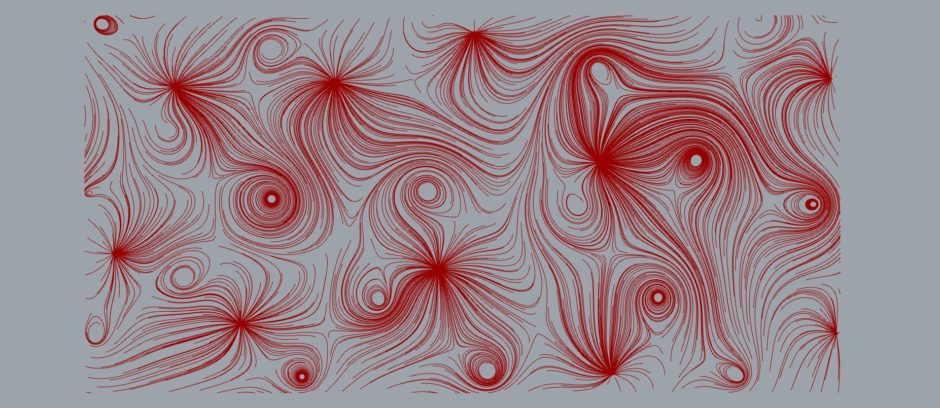
\includegraphics[width=23cm]{vektorfeld.jpeg}};
\end{scope}

\end{scope}

\node at ({\einschlag+2*\gelenk+\ruecken+1.5*\breite},24.3)
	[color=white,scale=1]
	{\hbox to\hsize{\hfill%
	\sf \fontsize{24}{24}\selectfont Mathematisches Seminar}};

\node at ({\einschlag+2*\gelenk+\ruecken+1.5*\breite},21.9)
	[color=white,scale=1]
	{\hbox to\hsize{\hfill%
	\sf \fontsize{51}{51}\selectfont Felder}};

\node at ({\einschlag+2*\gelenk+\ruecken+1.5*\breite},19.7)
	[color=white,scale=1]
	{\hbox to\hsize{\hfill%
	\sf \fontsize{13}{5}\selectfont Andreas Müller}};

\ifthenelse{\boolean{teilnehmer}}{
\node at ({\einschlag+2*\gelenk+\ruecken+1.5*\breite},18.4)
	[color=white,scale=1]
	{\hbox to\hsize{\hfill%
	\sf \fontsize{13}{5}\selectfont
	Orlando Ingram,
	Cassandra Sutton,
	Shelley Kim,
	Israel Romero
	}};

\node at ({\einschlag+2*\gelenk+\ruecken+1.5*\breite},17.75)
	[color=white,scale=1]
	{\hbox to\hsize{\hfill%
	\sf \fontsize{13}{5}\selectfont
	Charlie Mccoy,
	Tabitha Moore,
	Wendell Reynolds,
	Marion Higgins
	}};

\node at ({\einschlag+2*\gelenk+\ruecken+1.5*\breite},17.1)
	[color=white,scale=1]
	{\hbox to\hsize{\hfill%
	\sf \fontsize{13}{5}\selectfont
	Alexander Blake,
	Kirk Rodriguez,
	Caleb Mcdaniel,
	Mack Rice
	}};
 
\node at ({\einschlag+2*\gelenk+\ruecken+1.5*\breite},16.45)
	[color=white,scale=1]
	{\hbox to\hsize{\hfill%
	\sf \fontsize{13}{5}\selectfont
	Nathan Stewart,
	Kristi Cummings,
	Dave Munoz,
	Isaac Spencer
	}};

\node at ({\einschlag+2*\gelenk+\ruecken+1.5*\breite},15.8)
	[color=white,scale=1]
	{\hbox to\hsize{\hfill%
	\sf \fontsize{13}{5}\selectfont
	Dwayne Ray
	}};

\node at ({\einschlag+2*\gelenk+\ruecken+1.5*\breite},15.15)
	[color=white,scale=1]
	{\hbox to\hsize{\hfill%
	\sf \fontsize{13}{5}\selectfont
	}};

\node at ({\einschlag+2*\gelenk+\ruecken+1.5*\breite},14.5)
	[color=white,scale=1]
	{\hbox to\hsize{\hfill%
	\sf \fontsize{13}{5}\selectfont
	}};

}{}
 
%\node at (0,3) [color=white] {\sf \LARGE Mathematisches Seminar 2017};

% Rücken
\node at ({\bogenbreite/2 + 0.00},18.5) [color=white,rotate=-90]
	{\sf\fontsize{35}{0}\selectfont Felder\strut};

% Buchrückseite
\node at ({\einschlag+0.5*\breite},18.6) [color=white] {\sf
\fontsize{13}{16}\selectfont
\vbox{%
\parindent=0pt
%\raggedright
Das Mathematische Seminar der Ostschweizer Fachhochschule
in Rapperswil hat sich im Frühjahrssemester 2025 dem Thema
Felder
zugewandt.
Ziel war, die mathematischen Grundkonzepte und Gemeinsamkeiten 
von Vektor- und Skalarfeldern in Physik und Technik zu ergründen.
Dieses Buch bringt das Skript des Vorlesungsteils mit den von den
Seminarteilnehmern beigetragenen Seminararbeiten zusammen.

\medskip

%Zum Umschlagbild: Eine Wendeltreppe entsteht aus horizontalen Treppenstufen,
%die spiralförmig um die vertikale Achse angeordnet sind.
%Sie bilden eine Wendelfläche oder Helikoide.
%In Kapitel~17 wird gezeigt, dass sie auch eine Minimalfläche ist, 
%also die Form, die eine Seifenhaut annimmt, die sich zwischen einem
%spiralförmig gebogenen Draht und einer Achse aufspannt.
}};

\def\qrbreite{3}
\def\qrrightoffset{0}
\def\qrbottomoffset{1.5}

\fill[color=white]
        ({\einschlag+(\breite+13.6)/2-\qrbreite-0.1},{\einschlag+\qrbottomoffset-0.1})
        rectangle
        ({\einschlag+(\breite+13.6)/2+0.1},{\einschlag+\qrbottomoffset+\qrbreite+0.1});

\node at ({\einschlag+(\breite+13.6)/2-\qrbreite/2},{\einschlag+\qrbottomoffset+\qrbreite/2}) {
\qrcode[height=3cm]{https://mathsem.ch/jahre/2025}
};
\node at ({\einschlag+(\breite+13.6)/2-\qrbreite/2},{\einschlag+\qrbottomoffset+\qrbreite/2}) {

\includegraphics[width=10mm]{mathman.png}
};

\ifthenelse{\boolean{guidelines}}{
\draw[white] (0,{\einschlag})--({\bogenbreite},{\einschlag});
\draw[white] (0,{\bogenhoehe-\einschlag})--({\bogenbreite},{\bogenhoehe-\einschlag});

\draw[white] ({\einschlag},0)--({\einschlag},{\bogenhoehe});
\draw[white] ({\einschlag+\breite},0)--({\einschlag+\breite},{\bogenhoehe});
\draw[white] ({\einschlag+\breite+\gelenk},0)--({\einschlag+\breite+\gelenk},{\bogenhoehe});
\draw[white] ({\bogenbreite-\einschlag-\breite-\gelenk},0)--({\bogenbreite-\einschlag-\breite-\gelenk},{\bogenhoehe});
\draw[white] ({\bogenbreite-\einschlag-\breite},0)--({\bogenbreite-\einschlag-\breite},{\bogenhoehe});
\draw[white] ({\bogenbreite-\einschlag},0)--({\bogenbreite-\einschlag},{\bogenhoehe});
}{}

\end{tikzpicture}
\end{document}
